\documentclass[aspectratio=169,12pt]{beamer}

% ── Theme ──
\usetheme{Madrid}
\usecolortheme{whale}
\setbeamertemplate{navigation symbols}{}
\setbeamertemplate{footline}{%
  \leavevmode\hbox{%
    \begin{beamercolorbox}[wd=.33\paperwidth,ht=2.5ex,dp=1ex,center]{author in head/foot}%
      \usebeamerfont{author in head/foot}\insertshortauthor
    \end{beamercolorbox}%
    \begin{beamercolorbox}[wd=.34\paperwidth,ht=2.5ex,dp=1ex,center]{title in head/foot}%
      \usebeamerfont{title in head/foot}\insertshorttitle
    \end{beamercolorbox}%
    \begin{beamercolorbox}[wd=.33\paperwidth,ht=2.5ex,dp=1ex,right]{date in head/foot}%
      \usebeamerfont{date in head/foot}\insertframenumber{}/\inserttotalframenumber\hspace*{2ex}
    \end{beamercolorbox}}%
}

% ── Packages ──
\usepackage{booktabs}
\usepackage{amsmath,amssymb}
\usepackage{tikz}
\usetikzlibrary{arrows.meta,positioning,shapes.geometric,calc}
\usepackage{xcolor}
\usepackage{colortbl}

% ── Colors ──
\definecolor{dstblue}{HTML}{2C5F8A}
\definecolor{dstgreen}{HTML}{2E8B57}
\definecolor{dstorange}{HTML}{D4760A}
\definecolor{dstred}{HTML}{C44E52}
\definecolor{dstpurple}{HTML}{7B4F9D}
\definecolor{dstgray}{HTML}{666666}
\definecolor{highlight}{HTML}{D4EDDA}
\definecolor{lightblue}{HTML}{E8F0FE}
\definecolor{lightorange}{HTML}{FFF3E0}
\definecolor{lightred}{HTML}{FDEDEC}
\definecolor{lightpurple}{HTML}{F3E5F5}

% ── Title ──
\title[DSGD++ Rule Induction]{Uncertainty-Driven Rule Induction\\for Dempster-Shafer Classifiers}
\subtitle{Methodology and Experimental Design}
\author[H.~Tarkhanyan]{Hayk Tarkhanyan}
\date{April 2026}

\begin{document}

% ════════════════════════════════════════════
\begin{frame}
\titlepage
\end{frame}

% ════════════════════════════════════════════
\begin{frame}{Outline}
\tableofcontents
\end{frame}


%%%%%%%%%%%%%%%%%%%%%%%%%%%%%%%%%%%%%%%%%%%%%
\section{Background: Dempster-Shafer Theory}
%%%%%%%%%%%%%%%%%%%%%%%%%%%%%%%%%%%%%%%%%%%%%

% ────────────────────────────────────────────
\begin{frame}{Mass Assignment Functions}

\textbf{Frame of discernment:} $\Omega = \{c_1, c_2, \ldots, c_k\}$

\vspace{1em}
A \textbf{Mass Assignment Function} distributes belief across subsets of $\Omega$:
$$m: 2^\Omega \rightarrow [0,1] \qquad \sum_{A \subseteq \Omega} m(A) = 1$$

\vspace{1em}
For classification we use \textbf{singletons} + \textbf{full frame}:

\vspace{0.5em}
\begin{center}
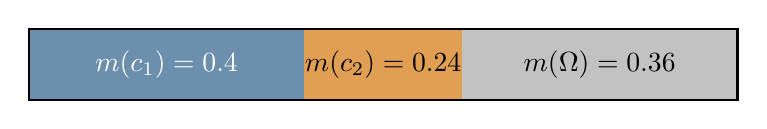
\begin{tikzpicture}
\draw[fill=dstblue!70, draw=none] (0,0) rectangle (3.5,0.9);
\draw[fill=dstorange!70, draw=none] (3.5,0) rectangle (5.5,0.9);
\draw[fill=dstgray!40, draw=none] (5.5,0) rectangle (9.0,0.9);
\draw[thick] (0,0) rectangle (9.0,0.9);
\node at (1.75,0.45) {\color{white}\textbf{$m(c_1) = 0.4$}};
\node at (4.5,0.45) {\textbf{$m(c_2) = 0.24$}};
\node at (7.25,0.45) {$m(\Omega) = 0.36$};
\end{tikzpicture}
\end{center}

\vspace{1em}
$m(\Omega)$ represents \textcolor{dstred}{uncertainty} --- belief not committed to any class.

\end{frame}

% ────────────────────────────────────────────
\begin{frame}{Belief and Plausibility}

From the MAF we derive two measures for any class $c_j$:

\vspace{1em}
$$\text{Bel}(c_j) = m(c_j) \qquad \text{Pl}(c_j) = m(c_j) + m(\Omega)$$

\vspace{1em}
\textbf{Interpretation:} The true probability of class $c_j$ lies in:
$$P(c_j) \in [\text{Bel}(c_j),\; \text{Pl}(c_j)]$$

\vspace{1em}
\textbf{Example:} With $m(+) = 0.4$, $m(-) = 0.24$, $m(\Omega) = 0.36$:
\begin{itemize}
    \item $P(+) \in [0.40,\; 0.76]$ --- likely positive but uncertain
    \item $P(-) \in [0.24,\; 0.60]$ --- less likely but plausible
\end{itemize}

\vspace{0.5em}
The \textbf{width} of the interval reflects model uncertainty.

\end{frame}

% ────────────────────────────────────────────
\begin{frame}{Dempster's Rule of Combination}

Combines \textbf{independent} evidence sources $m_1$ and $m_2$:

$$m_{1 \oplus 2}(A) = \frac{1}{1 - K}\sum_{\substack{B \cap C = A}} m_1(B) \cdot m_2(C)$$

\vspace{0.3em}
where $K = \sum_{B \cap C = \emptyset} m_1(B) \cdot m_2(C)$ measures conflict.

\vspace{1em}
\textbf{Key properties:}
\begin{itemize}
    \item \textbf{Commutative:} order of sources doesn't matter
    \item \textbf{Associative:} can chain multiple sources
    \item \textbf{Identity:} combining with $m(\Omega)=1$ returns the other source unchanged
\end{itemize}

\vspace{0.5em}
Agreeing sources $\rightarrow$ stronger belief. \quad Conflicting sources $\rightarrow$ higher $K$.

\end{frame}


%%%%%%%%%%%%%%%%%%%%%%%%%%%%%%%%%%%%%%%%%%%%%
\section{DSGD++ Classifier}
%%%%%%%%%%%%%%%%%%%%%%%%%%%%%%%%%%%%%%%%%%%%%

% ────────────────────────────────────────────
\begin{frame}{DSGD++ Overview}

\textbf{Idea:} Each rule is an evidence source with a learnable MAF.

\vspace{1em}
\begin{center}
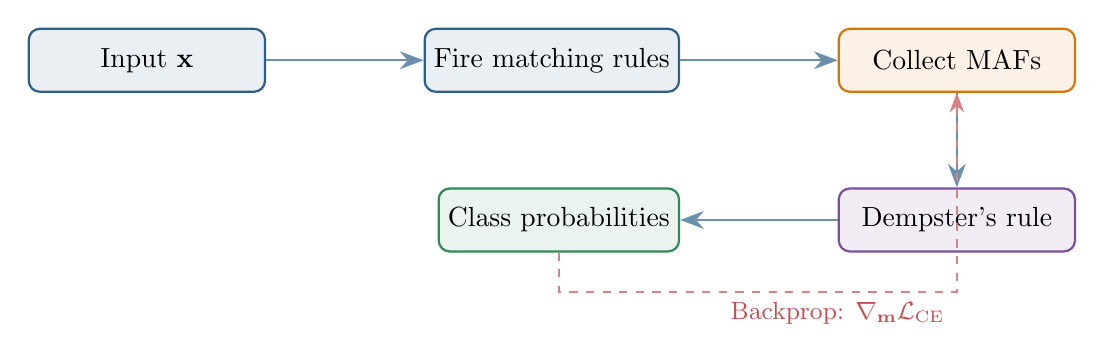
\begin{tikzpicture}[
    node distance=1.0cm and 2.0cm,
    box/.style={rectangle, draw=#1, fill=#1!10, rounded corners=4pt,
                minimum width=3.0cm, minimum height=0.8cm, font=\normalsize,
                align=center, thick},
    box/.default=dstblue,
    arr/.style={-{Stealth[length=3mm]}, thick, dstblue!70}
]
\node[box] (input) {Input $\mathbf{x}$};
\node[box, right=2cm of input] (fire) {Fire matching rules};
\node[box=dstorange, right=2cm of fire] (mafs) {Collect MAFs};
\node[box=dstpurple, below=1.2cm of mafs] (combine) {Dempster's rule};
\node[box=dstgreen, left=2cm of combine] (output) {Class probabilities};

\draw[arr] (input) -- (fire);
\draw[arr] (fire) -- (mafs);
\draw[arr] (mafs) -- (combine);
\draw[arr] (combine) -- (output);

\draw[-{Stealth[length=2.5mm]}, thick, dstred!70, dashed]
    (output.south) -- ++(0,-0.5) -| node[below, pos=0.35, font=\small, dstred]
    {Backprop: $\nabla_\mathbf{m}\mathcal{L}_\text{CE}$} (mafs.south);
\end{tikzpicture}
\end{center}

\vspace{0.5em}
\begin{itemize}
    \item \textbf{Rules} are fixed Boolean predicates (not learned)
    \item \textbf{MAFs} are the learnable parameters (optimized by Adam)
    \item After each step: \texttt{normalize()} ensures $m_i \geq 0$ and $\sum m_i \leq 1$
\end{itemize}

\end{frame}

% ────────────────────────────────────────────
\begin{frame}{Forward Pass: Commonality Trick}

Direct computation of Dempster's rule is expensive.

\vspace{1em}
\textbf{Solution:} Convert masses to \textit{commonalities} and multiply.

\vspace{0.5em}
For each fired rule $i$ with masses $(m_{c_1}^{(i)}, \ldots, m_{c_k}^{(i)}, m_\Theta^{(i)})$:

$$q_{c_j}^{(i)} = m_{c_j}^{(i)} + m_\Theta^{(i)}$$

\vspace{0.5em}
Combine all $n$ fired rules by element-wise product:
$$Q_{c_j} = \prod_{i=1}^{n} q_{c_j}^{(i)}$$

\vspace{0.5em}
Normalize to get class probabilities:
$$P(c_j | \mathbf{x}) = \frac{Q_{c_j}}{\sum_{j'} Q_{c_{j'}}}$$

\vspace{0.5em}
This is a single matrix multiply + normalize --- fully differentiable in PyTorch.

\end{frame}

% ────────────────────────────────────────────
\begin{frame}{Base Rule Generation}

For each feature $f$, compute mean $\mu_f$ and std $\sigma_f$ on training data.

\vspace{0.5em}
With $B = 2$ breaks at normal quantile positions $z_1, z_2$, generate 3 rules:

\vspace{1em}
\begin{center}
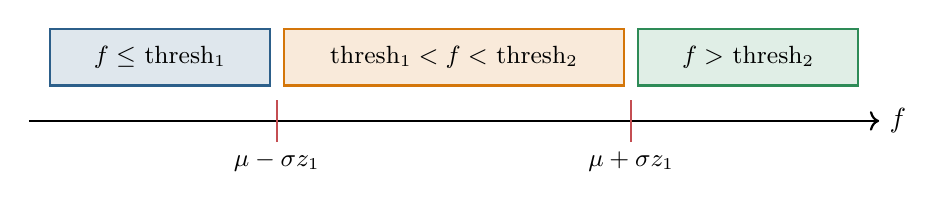
\begin{tikzpicture}[scale=0.9]
% Number line
\draw[thick, ->] (0,0) -- (12,0) node[right] {$f$};

% Break points
\draw[thick, dstred] (3.5,-0.3) -- (3.5,0.3);
\draw[thick, dstred] (8.5,-0.3) -- (8.5,0.3);
\node[below, font=\small] at (3.5,-0.3) {$\mu - \sigma z_1$};
\node[below, font=\small] at (8.5,-0.3) {$\mu + \sigma z_1$};

% Regions
\draw[thick, dstblue, fill=dstblue!15] (0.3,0.5) rectangle (3.4,1.3);
\node[font=\small] at (1.85,0.9) {$f \leq$ thresh$_1$};

\draw[thick, dstorange, fill=dstorange!15] (3.6,0.5) rectangle (8.4,1.3);
\node[font=\small] at (6.0,0.9) {thresh$_1 < f <$ thresh$_2$};

\draw[thick, dstgreen, fill=dstgreen!15] (8.6,0.5) rectangle (11.7,1.3);
\node[font=\small] at (10.15,0.9) {$f >$ thresh$_2$};
\end{tikzpicture}
\end{center}

\vspace{1em}
Total: $d \times (B + 1)$ rules for $d$ features.

\vspace{0.5em}
Example: 13 features $\times$ 3 rules = 39 base rules for heart disease.

\end{frame}

% ────────────────────────────────────────────
\begin{frame}{MAF Initialization}

How do we set the initial masses before training?

\vspace{1.5em}
\textbf{Random} (default):
\begin{itemize}
    \item Small random mass per class, high uncertainty ($m_\Theta \approx 0.8$)
    \item Lets gradient descent learn everything from scratch
\end{itemize}

\vspace{1em}
\textbf{Clustering-based:}
\begin{itemize}
    \item Run KMeans on the training data
    \item For each rule, measure how close covered samples are to cluster centroids
    \item Initialize $m_{c_j}$ proportional to cluster membership confidence
    \item Gives the optimizer a better starting point
\end{itemize}

\vspace{1em}
\textbf{Both are then refined by gradient descent} --- the initialization
affects convergence speed but the final accuracy is often similar.

\end{frame}


%%%%%%%%%%%%%%%%%%%%%%%%%%%%%%%%%%%%%%%%%%%%%
\section{E1: Rule Source Comparison}
%%%%%%%%%%%%%%%%%%%%%%%%%%%%%%%%%%%%%%%%%%%%%

% ────────────────────────────────────────────
\begin{frame}{E1: Motivation}

Base rules (single-feature thresholds) have a fundamental limitation:

\vspace{1em}
\textbf{They cannot capture feature interactions.}

\vspace{1em}
A rule like ``glucose $>$ 140'' is useful, but the combination\\
``glucose $>$ 140 \textbf{AND} BMI $>$ 30'' is far more predictive for diabetes.

\vspace{1.5em}
\textbf{Research question:}\\
If we mine conjunctive rules from external algorithms and add them\\
to DSGD++, which mining source helps the most?

\end{frame}

% ────────────────────────────────────────────
\begin{frame}{E1: Three Rule Miners}

\textbf{SkopeRules} (bagged stumps):
\begin{itemize}
    \item Trains many shallow decision trees, extracts rules meeting precision/recall thresholds
    \item Produces many diverse conjunctive rules
\end{itemize}

\vspace{0.8em}
\textbf{RIPPER} (sequential covering):
\begin{itemize}
    \item Greedy algorithm: find best rule, remove covered samples, repeat
    \item Produces compact, non-overlapping rule sets
\end{itemize}

\vspace{0.8em}
\textbf{Decision Tree} (leaf-path extraction):
\begin{itemize}
    \item Train a shallow tree (depth 3--4), extract root-to-leaf paths as rules
    \item Rules have good coverage and purity guarantees
\end{itemize}

\end{frame}

% ────────────────────────────────────────────
\begin{frame}{E1: Protocol}

\begin{enumerate}
    \item Generate base single-feature rules ($d \times 3$ rules)

    \vspace{0.5em}
    \item For each miner separately:
    \begin{enumerate}
        \item[a.] Fit the miner on training data
        \item[b.] Extract rules as strings (e.g., \texttt{``X[2] > 0.5 and X[5] <= 1.3''})
        \item[c.] Parse and convert to DSRule lambda functions
        \item[d.] Add to DSGD++ model with random MAF initialization
    \end{enumerate}

    \vspace{0.5em}
    \item Train DSGD++ (500 epochs, cross-entropy, Adam)

    \vspace{0.5em}
    \item Evaluate on held-out test set (accuracy, F1, AUC)
\end{enumerate}

\vspace{1em}
\textbf{Baseline:} DSGD++ with only base rules (no mined rules).

\end{frame}


%%%%%%%%%%%%%%%%%%%%%%%%%%%%%%%%%%%%%%%%%%%%%
\section{E2: Iterative Uncertainty-Guided Refinement}
%%%%%%%%%%%%%%%%%%%%%%%%%%%%%%%%%%%%%%%%%%%%%

% ────────────────────────────────────────────
\begin{frame}{E2: Core Idea}

\begin{center}
\Large
\textcolor{dstblue}{Use DSGD++'s own uncertainty to guide rule mining.}
\end{center}

\vspace{1.5em}
After training, some rules have high $m_\Theta$ --- the model is
uncertain about the samples those rules cover.

\vspace{1em}
Instead of mining rules globally, we mine rules \textbf{specifically for}
the uncertain regions.

\vspace{1em}
Then we retrain and check if uncertainty decreased.

\vspace{1em}
This creates a \textbf{closed feedback loop}: uncertainty drives rule creation,
which reduces uncertainty.

\end{frame}

% ────────────────────────────────────────────
\begin{frame}{E2: Rule Confidence Score}

After training, each rule $r$ has learned masses
$\mathbf{m}_r = (m_{c_1}, \ldots, m_{c_k}, m_\Theta)$.

\vspace{1.5em}
\textbf{Confidence score:}
$$c_r = \underbrace{\max_{j}\; m_{c_j}}_{\text{strongest class belief}}
      \;\times\;
      \underbrace{(1 - m_\Theta)}_{\text{certainty}}$$

\vspace{1.5em}
\begin{itemize}
    \item $c_r \approx 1$: rule is confident and informative
    \item $c_r < 0.3$: rule is \textbf{weak} --- covers an ambiguous region
\end{itemize}

\vspace{1em}
\textbf{Example:} $\mathbf{m} = (0.15, 0.10, 0.75)$
$\implies c_r = 0.15 \times 0.25 = 0.04$ \quad (very weak)

\end{frame}

% ────────────────────────────────────────────
\begin{frame}{E2: The Iterative Loop}

\begin{center}
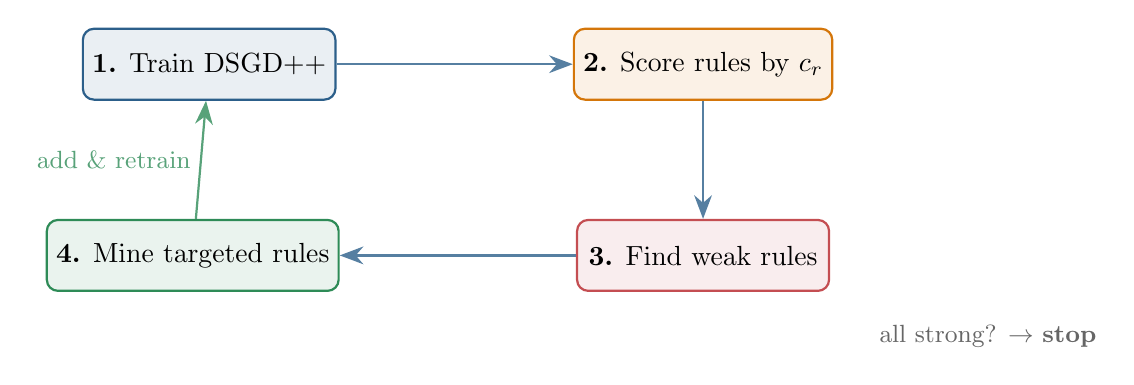
\begin{tikzpicture}[
    node distance=1.2cm and 2.5cm,
    box/.style={rectangle, draw=#1, fill=#1!10, rounded corners=4pt,
                minimum width=3.2cm, minimum height=0.9cm, font=\normalsize,
                align=center, thick},
    box/.default=dstblue,
    arr/.style={-{Stealth[length=3mm]}, thick, dstblue!80}
]
\node[box=dstblue] (train) {\textbf{1.} Train DSGD++};
\node[box=dstorange, right=3cm of train] (score) {\textbf{2.} Score rules by $c_r$};
\node[box=dstred, below=1.5cm of score] (weak) {\textbf{3.} Find weak rules};
\node[box=dstgreen, left=3cm of weak] (mine) {\textbf{4.} Mine targeted rules};

\draw[arr] (train) -- (score);
\draw[arr] (score) -- (weak);
\draw[arr] (weak) -- (mine);
\draw[arr, dstgreen!80] (mine) -- node[left, font=\small] {add \& retrain} (train);

\node[below right=0.3cm and 0.5cm of weak, font=\small, dstgray]
    {all strong? $\rightarrow$ \textbf{stop}};
\end{tikzpicture}
\end{center}

\vspace{0.5em}
Maximum 3 iterations. Stop early if no weak rules remain.

\end{frame}

% ────────────────────────────────────────────
\begin{frame}{E2: Targeted Mining Details}

For each weak rule $r$ (sorted by confidence, weakest first):

\vspace{1em}
\begin{enumerate}
    \item \textbf{Collect covered samples:} $S_r = \{\mathbf{x} : r(\mathbf{x}) = \text{True}\}$

    \vspace{0.5em}
    \item \textbf{Skip if trivial:}
    \begin{itemize}
        \item $|S_r| < 10$ (too few samples to mine from)
        \item Region already pure (single class --- nothing to improve)
    \end{itemize}

    \vspace{0.5em}
    \item \textbf{Run miner on $S_r$ only} (not on full dataset)

    \vspace{0.5em}
    \item \textbf{Add up to 3 new rules} per weak rule
\end{enumerate}

\vspace{1em}
Process up to 10 weak rules per iteration.

\end{frame}

% ────────────────────────────────────────────
\begin{frame}{E2: Rule Cap and Safeguards}

\textbf{Problem:} Iterative mining could explode the rule count.

\vspace{1em}
\textbf{Solution: Global rule cap} at $3\times$ base rules.

\vspace{0.5em}
\begin{itemize}
    \item Example: 13 features $\times$ 3 = 39 base rules $\rightarrow$ cap at 117
    \item Once cap is reached, no more rules are added even if weak rules remain
\end{itemize}

\vspace{1.5em}
\textbf{Additional safeguards:}
\begin{itemize}
    \item Max 3 iterations (prevents infinite loops)
    \item Max 3 new rules per weak rule (prevents single-region flooding)
    \item Retraining after each iteration (all masses re-optimized jointly)
    \item Early stop if no new rules could be mined
\end{itemize}

\end{frame}


%%%%%%%%%%%%%%%%%%%%%%%%%%%%%%%%%%%%%%%%%%%%%
\section{E3: Multi-Source Rule Ensemble}
%%%%%%%%%%%%%%%%%%%%%%%%%%%%%%%%%%%%%%%%%%%%%

% ────────────────────────────────────────────
\begin{frame}{E3: Motivation}

E1 showed different miners excel on different datasets.

\vspace{1em}
\textbf{Can we combine rules from all miners at once?}

\vspace{1.5em}
In traditional ML, ensembles need careful weighting or stacking.

\vspace{0.5em}
In DSGD++, we have a natural solution:

\vspace{1em}
\begin{center}
\large
\textcolor{dstblue}{Dempster's rule was designed to combine\\
evidence from heterogeneous sources.}
\end{center}

\vspace{1em}
Each miner's rules get their own MAFs --- the model learns
how much to trust each source during training.

\end{frame}

% ────────────────────────────────────────────
\begin{frame}{E3: Protocol}

\begin{enumerate}
    \item Generate base single-feature rules

    \vspace{0.5em}
    \item Add rules from \textbf{all} miners simultaneously:
    \begin{itemize}
        \item SkopeRules (up to 10 rules)
        \item RIPPER (up to 10 rules)
        \item Decision Tree (depth 3, all leaf paths)
    \end{itemize}

    \vspace{0.5em}
    \item Each rule gets its own MAF --- initialized randomly

    \vspace{0.5em}
    \item Train DSGD++ jointly on the full rule set

    \vspace{0.5em}
    \item Evaluate on held-out test set
\end{enumerate}

\vspace{1em}
\textbf{Comparison:} Single-source (base rules only) vs.\ multi-source.

\vspace{0.5em}
No manual weighting needed --- gradient descent handles it.

\end{frame}


%%%%%%%%%%%%%%%%%%%%%%%%%%%%%%%%%%%%%%%%%%%%%
\section{E4: Pruning Pareto Frontier}
%%%%%%%%%%%%%%%%%%%%%%%%%%%%%%%%%%%%%%%%%%%%%

% ────────────────────────────────────────────
\begin{frame}{E4: Accuracy vs.\ Interpretability}

More rules $\rightarrow$ potentially better accuracy, but less interpretable.

\vspace{1em}
\textbf{Goal:} Find the sweet spot --- how many rules can we remove
while keeping accuracy?

\vspace{1.5em}
\textbf{Approach:}
\begin{enumerate}
    \item Train a full model with many rules (base + all mined)
    \item Compute confidence $c_r$ for every rule
    \item Sweep a threshold $\tau$ from 0 to 0.45
    \item For each $\tau$: deactivate rules with $c_r < \tau$, measure accuracy
    \item Plot: active rules vs.\ accuracy (Pareto frontier)
\end{enumerate}

\vspace{1em}
\textbf{Baseline:} Random pruning (remove random rules at same rates).

\end{frame}

% ────────────────────────────────────────────
\begin{frame}{E4: Why Confidence Pruning Works}

Rules with low $c_r$ contribute little to decisions:
\begin{itemize}
    \item High $m_\Theta$ means the rule's MAF is close to the identity element
    \item Combining with identity doesn't change the result
    \item Removing such rules has minimal effect on predictions
\end{itemize}

\vspace{1.5em}
\textbf{Confidence pruning vs.\ random pruning:}
\begin{itemize}
    \item Confidence pruning removes the least informative rules first
    \item Random pruning may accidentally remove important rules
    \item The gap between the two curves shows how much structure
          the confidence score captures
\end{itemize}

\end{frame}


%%%%%%%%%%%%%%%%%%%%%%%%%%%%%%%%%%%%%%%%%%%%%
\section{E5: Baselines}
%%%%%%%%%%%%%%%%%%%%%%%%%%%%%%%%%%%%%%%%%%%%%

% ────────────────────────────────────────────
\begin{frame}{E5: Baseline Models}

\textbf{Interpretable baselines} (fair comparison):
\begin{itemize}
    \item Decision Tree (depth 4, depth 8)
    \item RuleFit --- rules + linear model
    \item FIGS --- fast interpretable greedy tree sums
    \item RIPPER --- sequential covering
    \item SkopeRules --- rule extraction from bagged trees
    \item Greedy Rule List --- ordered if-then-else
\end{itemize}

\vspace{1em}
\textbf{Black-box baselines} (upper bound on performance):
\begin{itemize}
    \item Gradient Boosting (100 trees, depth 4)
    \item Random Forest (100 trees, depth 8)
    \item Logistic Regression
\end{itemize}

\vspace{0.5em}
Same train/test split, same seed (509) across all models.

\end{frame}


%%%%%%%%%%%%%%%%%%%%%%%%%%%%%%%%%%%%%%%%%%%%%
\section{MAF Initialization Comparison}
%%%%%%%%%%%%%%%%%%%%%%%%%%%%%%%%%%%%%%%%%%%%%

% ────────────────────────────────────────────
\begin{frame}{Random vs.\ Clustering Initialization}

\textbf{Question:} Does a better starting point for MAFs lead to better results?

\vspace{1.5em}
\textbf{Random init:}
\begin{itemize}
    \item $m_{c_j} \sim$ small random values, $m_\Theta \approx 0.8$
    \item Model starts with high uncertainty, learns everything via gradient descent
\end{itemize}

\vspace{1em}
\textbf{Clustering init:}
\begin{itemize}
    \item KMeans on training data $\rightarrow$ cluster distances
    \item For each rule: measure how well covered samples align with clusters
    \item Initialize $m_{c_j}$ proportional to cluster confidence
    \item Model starts closer to a good solution
\end{itemize}

\vspace{1em}
We run E1--E3 with \textbf{both initializations} on all 6 datasets,
saving results separately.

\end{frame}


%%%%%%%%%%%%%%%%%%%%%%%%%%%%%%%%%%%%%%%%%%%%%
\section{Datasets and Setup}
%%%%%%%%%%%%%%%%%%%%%%%%%%%%%%%%%%%%%%%%%%%%%

% ────────────────────────────────────────────
\begin{frame}{Datasets}

\begin{table}
\centering
\begin{tabular}{lrrrl}
\toprule
\textbf{Dataset} & \textbf{Samples} & \textbf{Features} & \textbf{Class ratio} & \textbf{Source} \\
\midrule
Heart Disease      & 303   & 13 & 54/46 & UCI \\
Breast Cancer      & 683   & 9  & 65/35 & UCI \\
Ionosphere         & 351   & 34 & 64/36 & UCI \\
PIMA Diabetes      & 768   & 8  & 65/35 & OpenML \\
QSAR Biodeg.       & 1{,}055 & 41 & 66/34 & UCI \\
Phoneme            & 5{,}404 & 5  & 71/29 & OpenML \\
\bottomrule
\end{tabular}
\end{table}

\vspace{1em}
\begin{itemize}
    \item All binary classification, all numeric features
    \item 70/30 stratified train/test split, seed = 509
    \item StandardScaler fit on training data only
\end{itemize}

\end{frame}

% ────────────────────────────────────────────
\begin{frame}{DSGD++ Configuration}

\begin{table}
\centering
\begin{tabular}{ll}
\toprule
\textbf{Parameter} & \textbf{Value} \\
\midrule
Max epochs & 500 \\
Optimizer & Adam \\
Learning rate & 0.005 \\
Loss function & Cross-entropy \\
Statistical breaks & 2 (3 rules per feature) \\
Rule cap (E2) & $3\times$ base rules \\
E2 max iterations & 3 \\
E2 uncertainty threshold & 0.3 \\
E2 max weak rules per iter & 10 \\
E2 max new rules per weak rule & 3 \\
\bottomrule
\end{tabular}
\end{table}

\end{frame}


%%%%%%%%%%%%%%%%%%%%%%%%%%%%%%%%%%%%%%%%%%%%%
\section{Summary}
%%%%%%%%%%%%%%%%%%%%%%%%%%%%%%%%%%%%%%%%%%%%%

% ────────────────────────────────────────────
\begin{frame}{Experiment Matrix}

\begin{center}
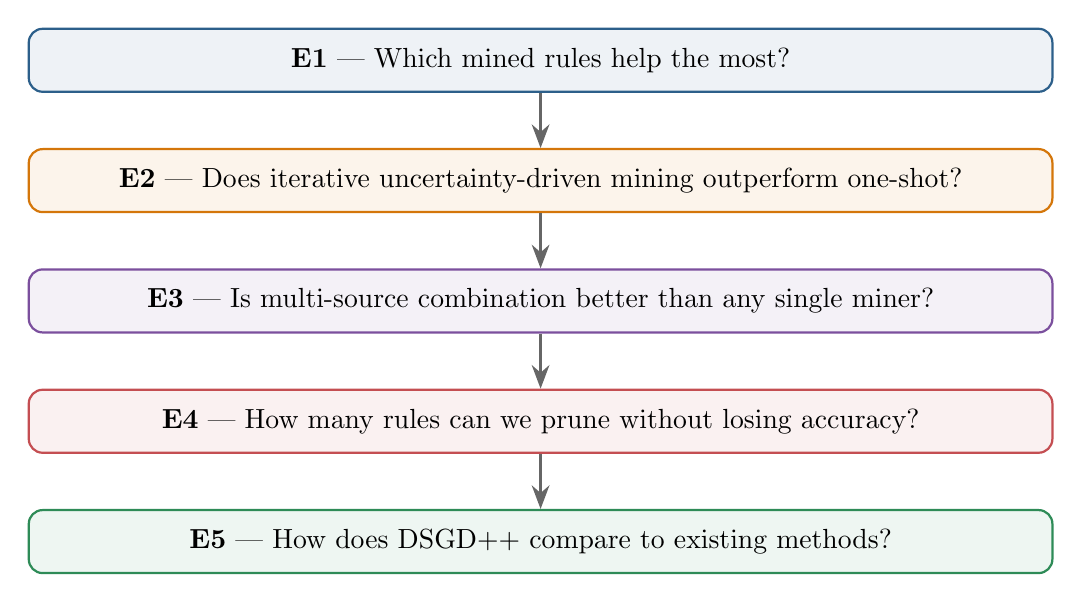
\begin{tikzpicture}[
    node distance=0.7cm,
    bigbox/.style={rectangle, draw=#1, fill=#1!8, rounded corners=5pt,
                   minimum width=13cm, minimum height=0.8cm,
                   font=\normalsize, align=center, thick},
    bigbox/.default=dstblue,
    arr/.style={-{Stealth[length=3mm]}, thick, dstgray}
]

\node[bigbox=dstblue] (e1) {\textbf{E1} --- Which mined rules help the most?};
\node[bigbox=dstorange, below=of e1] (e2) {\textbf{E2} --- Does iterative uncertainty-driven mining outperform one-shot?};
\node[bigbox=dstpurple, below=of e2] (e3) {\textbf{E3} --- Is multi-source combination better than any single miner?};
\node[bigbox=dstred, below=of e3] (e4) {\textbf{E4} --- How many rules can we prune without losing accuracy?};
\node[bigbox=dstgreen, below=of e4] (e5) {\textbf{E5} --- How does DSGD++ compare to existing methods?};

\draw[arr] (e1) -- (e2);
\draw[arr] (e2) -- (e3);
\draw[arr] (e3) -- (e4);
\draw[arr] (e4) -- (e5);

\end{tikzpicture}
\end{center}

\vspace{0.5em}
\centering
6 datasets $\times$ 5 experiments $\times$ 2 initializations = comprehensive evaluation.

\end{frame}

% ════════════════════════════════════════════
\begin{frame}{}
\begin{center}
\Huge\textcolor{dstblue}{Thank you}\\[1em]
\large Questions?\\[2em]
\normalsize
\textcolor{dstgray}{Code: \texttt{github.com/HaykTarkhanyan/dst\_research}}
\end{center}
\end{frame}

\end{document}
